\chapter{太阳城}

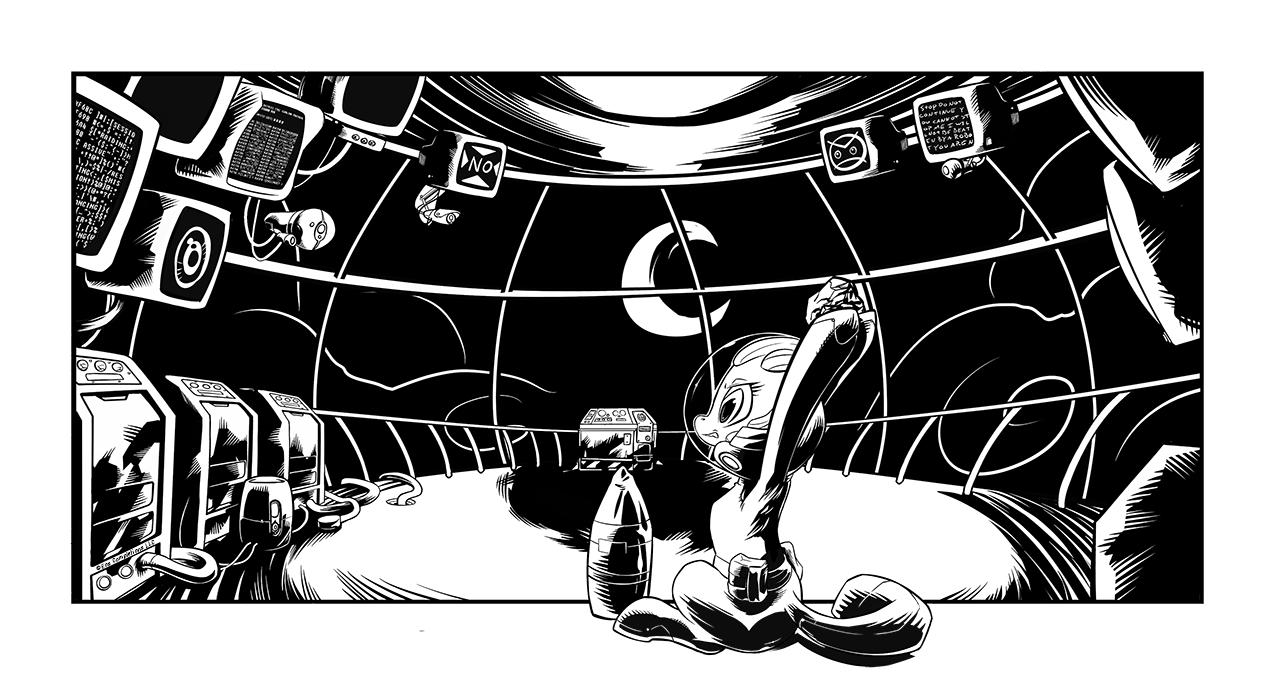
\includegraphics[width=\linewidth]{image09.png}

\begin{intro}
太阳城不只是一个小镇,它是小马们罪孽的救赎。
\end{intro}

\daytimeplace{7}{11:00 PM}{太阳城郊外,52号国道中段}{Sun City Suburbs, Big 52 SC Branch}

去城里的路非常远,帕比走到第一个房子边的时候,夜晚的黑暗已经笼罩了街道的每一个角落。太阳城中心社区被一大堆小小卫星城区包围着。但是每个窗户都黑漆漆一片,半点光亮也没有。帕比走过的建筑看起来都已经被拾荒者洗劫一空,只剩下一个个房子尸体般的空壳,就像是一片坟墓,一片曾经被叫做「家」的东西的坟墓。

帕比并不想承认她还有点怕黑,但是这个空旷的地方让她想起来小时候的各种鬼故事,「为什么小鸡要跑到这么可怕的地方惹麻烦?笨赫瑞!这里什么都没有,为什么还叫『城镇』?」

随着深入这个可怕的地方,帕比开始好奇,那些五颜六色的标志都去哪里了?虽然她没怎么在夜晚出去过,但是她很确定夜晚的城市不是这个样子……她想要一些音乐以此盖过夜晚阴风吹过空洞房屋发出的哀嚎,但是无线电一到太阳城附近就没有声音了,让帕比感觉到又孤单又害怕。「呐,声……声音先生……你还在吗?」

回答帕比的只有一堆毫无意义的沙沙声。

「{\mt 兹兹……危险……沙沙沙……变……兹兹……电……沙沙沙……可能……哔哔……影响……哗哗哗……思考。}」

「唉,他又生气了……」幼驹皱着眉头继续走着,头盔的HUD开始显示文字的警告信息,但是密密麻麻的字幕活像是蚂蚁,而且滚动速度快到帕比根本没办法看清。小雌驹觉得自己孤立无援——无线电坏了,声音先生不见了。就像那些可怕的夜晚,她想要睡觉但是屋子太黑太可怕,她不停地叫着妈妈,直到妈妈过来抱起她抚摸着她,把她哄安心。帕比想要唱点儿什么壮胆,但是在这种黑漆漆的地方她只能想起「邪恶女妖」啥的歌,完全没有什么帮助。

帕比走过迷宫一般空旷的街道,蹄声的回音让她觉得毛骨悚然。每一个空洞的窗户都反射着她双眸里明亮的粉色鬼火,那是什么?或许马尾伯爵又从坟墓里面爬出来了?而且她觉得这个时候就连马尾伯爵都不那么可怕了……远处传来一阵不可状名的尖叫声吓得幼驹僵立在原地,她后蹄一软直接坐在了马路上。

「那……那……那……那……那……那……是啥?」

打烂坏蛋机器和追着妈妈一点都不可怕,而尸鬼小马虽然看起来很惊悚但是她至少知道自己可以打什么……但是这里完全不一样——一个空无一物的城市,到处都是闹鬼的房子和发出怪声的街道,她为什么想到鬼怪幽灵?不要幽灵!坏幽灵!为什么她要离开红旗子的小路,漂漂姐姐明明说她不要离开那条路,但是她必须来这里帮那个笨小鸡。但是现在这里又黑又可怕,帕比超想念丝尾小姐。

小幼驹趴在路上耷拉着耳朵,尽力假装自己是路上的一块石头。

「新……新……新……新……计划!我们在这里等明……」

另一阵声音在空旷的街道回响着,好像是幽灵的哀嚎一般。

「……天……啊啊啊啊呀呀呀呀!」帕比撒开四蹄,风驰电掣,就像在落叶赛跑上的云宝黛西那样一溜烟飞奔出去。

「新计划!我们出城等天亮!」

\begin{center}
太阳城1分——帕比0分
\end{center}

\horizonline

\daytimeplace{8}{8:00 AM}{太阳城郊外,52号国道中段}{Sun City, Big 52 SC Branch}

天亮之后,这个城市看起来和盐块城差不多,甚至比得上中心城,一点儿也不可怕……就是有点儿……呃……丑。帕比在想为什么昨晚自己那么害怕,她真是个笨小孩。

「看吧,声音先生,这里没什么好怕的!就是另一个城市,到处都是破房子和烂马路还有……」帕比忽然看见有什么东西从头上飞过,「还有漂漂翔马们\footnote{翔马们 (Peggysuses):天马这个单词的复数就连很多英语母语的人都会搞错}!好棒!」

幼驹撒欢跑了起来,追着那个飞行的影子。「喂!喂喂喂!漂漂翔马们等等我……等等噗……」抬头看着天跑的小幼驹完全没有看前面,径直撞进另一个走在街上的陆马怀里。

「哎呦……你为什么不看路啊!我先从这里跑的!」

那个棕毛黑鬃的成年陆马似乎正背着一大堆砖块和其它建筑材料,不过现在已经被帕比撞得散落一地,帕比心中一惊然后立刻打算在那个老马生气之前溜走,但是他只是低头开始默默地把砖块捡回去。

「哼!这下知道教训了吧……别站在路中间和一个笨雕像一样!」帕比吐出舌头做鬼脸,但是她发现那个陆马根本没有在意她。他看起来只是有点……怎么说……

「呃,抱歉先生,您没听到么,我是快乐帕比,我在找我的妈妈……虽然通常是这样,不过今天我是来救我的朋友赫瑞,听说她在这里惹上麻烦,但是我又不知道是什么样的麻烦,你有看到她么,她有一个喙而且长着毛,看起来像是一只小鸡但是又不喜欢我叫她小鸡,但是我叫她小鸡又不是她想的那个小鸡,不管怎么说她都看起来像是小鸡,对了哦,我还见过斑马,我不知道为什么小马都不喜欢斑马而且那个斑马也不喜欢我们叫她斑马或许这就和小鸡不喜欢别人叫她小鸡一个道理……」

帕比紧紧跟着那个陆马,但是陆马却一言不发的,他捡起掉下的所有东西,然后走向城中心。帕比可以看见清楚看到那些完全被搜刮一空的房子似乎是城市的外围,就像是大概200米左右的无马区,但是城市里面却不一样,似乎小马们正将城市外面的房子一砖一瓦地拆散,然后再修葺好城市中心的房屋。

帕比停下来,看着面前这个在晨光中冉冉发光的城市赞叹道,「哇哦,你们还真有个漂亮的小镇!超赞!」

就在小雌驹面前展现的是如同往昔记忆之中的城市一样——有很多粉刷得很漂亮的小房子,屋顶上有门洞,门上也没钉着木板,各式各样的小马搬着各种东西忙碌着,看起来是个非常活跃的社区:大家都在忙着做什么事情,就算是幼驹和天马也是,有漂漂房子,漂漂飞天马车,就算是花园看起来也不是枯黄而是翠绿色,甚至还有绿树!帕比觉得这个地方完全可以打60分,不过,不管怎么说这可是这么长的旅途以来,第一个她觉得值得打分的地方!

「乐乐姐绝对大错特错!」帕比跟着她刚刚撞上的棕色小马,「小马真的是太喜欢这里所以不想回去了!事实再一次证明人家的正确性!哦哦,对了,说起来乐乐姐……呃……你好像不怎么喜欢说话……」不是不怎么,是完全不说话,所以帕比决定还是不管那个陆马,自己在这里逛逛。这个非常漂亮的城镇让她想起了妈咪带她去过的一些小镇,在废土游荡了八天之后,终于找到了一个美丽的小镇——即使这个小镇的小马都有些奇怪,让帕比觉得莫名其妙。

黄色的幼驹开始在这个城市里面探索,她看到一个狮鹫正蹲在屋顶上换着坏掉的瓦片,于是她大叫起来。「嘿!小鸡小姐!你看到我的朋友赫瑞了吗?她也是个小鸡!」但是,完全没有回答,这个地方的小马不是全都聋了,就是都非常不友善。

然后帕比看到一个独角兽雌驹正在给树浇水,于是她走过去,「打扰一下漂漂姐姐,请问您看到一个叫赫瑞塔的小鸡吗?」还是没回答,幼驹开始觉得不耐烦了,很明显她一直没什么进展,「呃,她另一半是猫咪!」

独角兽丝毫不管帕比继续浇着水。不过帕比这一次绝不会这么简单放弃,她亲自走到了那个独角兽和树之间,直视着她那双……斜眼?

「呃……你的眼睛……好奇怪?」

那雌驹一脸茫然地斜眼呆立着,「你怎么做到的?」帕比好奇地坐在地上看着她,「怎么让两个眼睛同时去看不同的方向?」

幼驹又一次被完全忽略,雌驹转身想要绕开帕比,但是黄色的幼驹坚持不懈地站在独角兽和树之间,最后她直接把水浇在了帕比头上然后走开了。

帕比现在又湿又不开心,「我说,这样很不礼貌耶!这里的小马都怎么了?为什么不和人家说话?是我身上臭臭吗?」幼驹低头嗅嗅自己身上,但是她穿着防护服一点意义都没有。

幼驹继续在社区里面转了一上午,想要找到谁可以和她聊天。但是这里的每一个小马都一样,一脸斜眼白痴表情,而且完全不听她讲话。

帕比想起以前她妈妈不让她看的那种奇怪电影,地铁二零几几什么什么的……不管怎么说她偷偷看了,而且无聊得要死,这个城市也一样,就像之前那个狂欢到真的让你死的农场一样,这里是无聊到真的让你变石头的地方。

她继续深入探索着这个城市,虽然路上偶遇几个和帕比年龄相仿的幼驹,但是他们也一样只知道工作,完全没有在玩,帕比真的努力去交朋友了,她试着和他们玩钉马尾或者更有趣的游戏,比如说扮太空小马和番茄星人,但是那些孩子就是不理他,现在帕比觉得又寂寞又伤心。

「声音先生走了,赫瑞又不知道去哪了,这里的小马都装傻不理人家!这里是最烂的城市!如果一点乐趣都没有,要那些漂漂房子和绿树有什么用?为啥大家都这么奇怪?」帕比叹了口气,她想起来每个小镇都应该有一个镇长或者什么管事的小马,或许问他的话可以找到一些答案,这些小马一般都住在市中心之类的地方,在太阳城这里是在明显不过了——那些摩天大楼显而易见是市中心。

「看起来超简单!」帕比蹦蹦哒哒地走向那边,但是却发现自己正漂浮起来远离自己的目标。

「哎?」

幼驹转过身才发现有个成年小马叼着她的后脖子,就像抓小猫一样把她拎出城去。

「喂喂喂!放开我坏蛋!我想要去那个闪亮亮的高塔!我要见市长!超重要的!你这个斜眼笨蛋!你有听我的话吗?」

那小马把帕比丢在了城市边缘的荒芜地区,然后留下在那里大喊大叫的小幼驹走开了。

\begin{center}
太阳城2分——帕比0分
\end{center}


\horizonline

\daytimeplace{8}{2:00 PM}{太阳城,52号国道中段}{Sun City, Big 52 SC Branch}

帕比一脸凝重的神色看着那些忙碌的小马思索着:他们不想让她走进城里,但是她必须想办法进去……或许她需要一点聪明的『战术』比如说穿个墨西哥宽边帽和斗篷之类的?恩……这个点子似乎不错,但是现在去哪儿找个假胡子呢?

忽然,幼驹的注意力被一个天上飞过的影子吸引了,她早已经习惯了天马在天上飞来飞去,不过这次不一样,是一个狮鹫,一个穿着熟悉铠甲的小小……「赫瑞塔!喂喂!赫瑞……等等!」

不过即使是她的最好朋友也不理她,帕比虽然不太开心但是她正忙着想办法引起赫瑞塔的注意,于是她大喊:「石头!」「命运之石」出现在帕比蹄子上。

她摆了一个Pose慢慢瞄准,然后……「咻……」「正中靶心!」狮鹫发出一声惨叫然后从天上栽下来,就像是……呃……被石头打中一样。

「别担心,赫瑞,我在下面接着你呢!」

帕比飞奔起来,想要在她满是羽毛的朋友坠落之前接住她,同时赫瑞塔正在拼命地想要从失速状态改出,但是她被砸得晕晕乎乎的脑袋完全没办法反应,她只能瞄准一个看起来软乎的东西做落点……对哦,那个黄色的小点进入了她的视线,一个不停地喊叫和奔跑的小黄点。

「我接着呢,我接着呢,别担心我……」

噗……「哎呦!」

「哎呀!」

狮鹫晕晕乎乎地看着快乐帕比,然后大叫起来。

「帕比肏你娘的,你丫在这么危险的地方闲逛个屁啊?还不快给老娘滚!如果听到那个嗡嗡……」赫瑞塔忽然也变成了斜眼,然后不说话了,一缕血丝顺着她头上的伤口流下,她也没反应。

「赫瑞,终于找到你了!丝尾告诉我你有危险但是……嘿!你想去哪儿啊?」狮鹫张开翅膀,然后准备起飞,但是黄色的小雌驹紧紧抓着赫瑞的脖子不让她飞起来,「别想逃掉!我们要一起离开这个破地方,你和我一咿呀呀呀!」

赫瑞塔比帕比强壮很多,她似乎一点都不在意,用蛮力把她丢到一边然后飞起来,帕比在空中划了一个弧线然后大头朝下地栽倒了一堆碎石之中,又一次只剩她自己了。

「怎么……刚刚怎么回事?前几天我们还一起打败大坏蛋,现在她就只是骂我一顿然后就飞走了?这不公平!这一点都不公平!好吧,如果她不想当我的朋友,我也不当她的朋友!我要我的丝尾!」帕比跑向城市寻找着她的前朋友,但是马上又停下来想,「但是我已经把丝丝当礼物给她了,我不能要回礼物……但是我想要我的朋友回来,至少要一个回来!」帕比摇了摇头,「不!我要他们俩都回来!不要回丝尾和赫瑞我哪儿也不去!现在我需要一个更好的计划!」不过什么计划呢,白天这里到处都是小马不让她进去,而晚上这里又那么可……或许也没那么可怕,毕竟这里不是真的鬼城……

幼驹回到城外坐在那里看着那些不那么漂漂的小马毫无意识地忙碌工作,她想到一个好点子……现在她只需要捡回「命运之石」然后等待夜幕降临……帕比藏在一堆碎石头后面,等待着她出击的机会。

「很快……」

\begin{center}
太阳城3分——帕比0分
\end{center}

\horizonline

\daytimeplace{8}{9:00 PM}{太阳城市中心,52号国道中段}{Sun City Downtown, Big 52 SC Branch}

帕比小心地紧贴着地面,弓着身子慢慢地爬着,「看不到我,看不到我……」她低声喃喃自语着,就像是那些她妈妈说太黄太暴力不能看的漫画书上的英雄一样……有时候妈妈也很烦,不过那些都不是重点,她现在是个有重要任务在身的小马,她必须专注于她的超级潜行技巧——像一个影子一般在夜幕中行动!

穿着亮黄色外衣,头戴发亮粉色光芒金鱼缸的幼驹低声嘀嘀咕咕:「看不到我,看不到我……」

计划很简单:穿过敌方防线,然后找到这个地方的老大,然后告诉他这地方烂透了!顺便找到赫瑞,最后在夕阳中逃向远方,就像那个小马哥电影的主角一样——绝不回头看爆炸。不过现在第一事情就是,去爬上那个超级神秘的摩天大楼顶楼一探究竟——好吧,现实点说,至少从电梯上到那个摩天大楼楼顶。

整个城市在晚上都空空如也,所有小马都不知道去哪里了,大概是睡觉去了,不过既然帕比知道这里没有鬼,只有一些做鬼脸的马,所以这里也没那么可怕了。帕比慢慢深入城镇,这里看起来就像是有谁建造了一个全新的城镇,然后又搬走了一样,完全静悄悄。虽然小雌驹也没看过一个全新的城镇是什么样,不过她觉得差不了多少。

唯一帕比能看到亮光的地方,就是那个蘑菇型的高塔,微弱的蓝光从最顶层黑暗的窗户里面照射出来,时不时地闪烁几下。那个神秘的建筑在黑暗之中不断发出微弱的轰鸣声。就像是那些妈咪不让她碰的超级超级危险电什么设备?\py{我是认真的,帕比!帕比你有在听吗?请跟我一起说:这不是玩具,我绝对不会碰它!}

「看不到我,看不到我……」

小心地检查了高塔的底层,帕比发现这里没有窗口,只有一个黑暗的玻璃门,上面画着旭日科技的标志。帕比推了推门,又拉了拉,但是完全没有反应。最后她用力敲着门喊道:「喂,这不公平!我怎么潜入一个没有入口的地方啊?笨塔为什么不按照……那个啥……剧本来?我是主角呢,懂吗,懂吗?」最后帕比还是要用老办法解决问题。

「石头!」

那是一个玻璃门——不管什么时候幼驹在街上玩球的时候,即使你非常小心注意不要打碎玻璃,但还是会打碎玻璃,所以当你真的要打碎玻璃的时候,那简直是小菜一碟。不过帕比显然没有见过防弹玻璃,所以她多花了一点时间。

当那蠢玻璃门终于变成渣渣从门框上落下来的时候,帕比仔细研究了一下,那个玻璃和她头盔上用的玻璃类似,被打中的时候只会出现蜘蛛网一样的裂纹但是不会碎成碎片,幸好幼驹已经有了很多用石头砸东西的经验,对于这个强化玻璃也不过是多砸个一两百下而已。

幼驹喘着粗气跨入建筑之中,她已经等不及要探索新的秘密,所以忍不住咯咯笑起来。边笑边唱道……

\begin{song}
你最好小心,你最好别哭!

You better watch out, you better not cry!

\medskip

你最好别噘嘴,我告诉你为什么:

You better not pout, 'cause I'm telling you why:

\medskip

快乐帕比要来镇上咯!\footnote{《圣诞老人进城》,一首美国经典圣诞歌}

Puppysmiles is coming to town.
\end{song}

这里虽然没有任何听众,不过小雌驹觉得最好要有,在她经历这么多麻烦之后,她要好好骂那个坏镇长一顿,让他知道这个小镇到底有多烂!

当幼驹来到大厅中央的大桌子之后,天花板上的一盏红灯开始闪烁起来并传来一阵电子语音……

「{\mt 警告,未授权自动机入侵,所有工作人员请呆在原地等待警报解除。}」

帕比完全不知道自动机啥的是什么意思,不过她知道这句话代表了什么——坏机器要来了。「喂,我劝你别来欺负我哦,人家可是有石头的!懂咩?」幼驹拿着她最喜欢的武器对着空无一物的走廊挥舞着,不过马上两门炮塔就冒了出来,但是它们只发出空膛的咔嗒声,帕比疑惑地看着炮塔,然后走过去戳着它。

「这才像话,你最好乖乖的!」小雌驹吐舌头做了个鬼脸,然后走向电梯,不过电梯闪着红灯根本动也不动。帕比就知道,所以她只好走向楼梯井,不过她继续唱起来。

\begin{song}
她要仔细检查清单两次,

She's making a list, and checking it twice!

\medskip

她要找出谁是好孩子,谁是坏孩子,

She's gonna find out who's naughty and nice.

\medskip

快乐帕比要来镇上咯。

Puppysmiles is coming to town.
\end{song}

长长的楼梯穿过很多楼层,里面全都是干净的空屋子,好像里面已经准备好接收运来的家具一样。

在楼梯的顶端是一扇强化门,上面还是标着旭日公司的标志,帕比用蹄子敲着门,「喂,我是快乐帕比!我要见镇长!这小镇烂透了!」里面还是没有回答,于是她更加用力地敲着门,更加大声地喊着:「不准无视我!在这个破地方大家都不理我!连我最好的朋友,连声音先生也不理我!为什么你们要不理我,你们不想做朋友吗?」

还是没有任何回复,但是帕比知道镇长在里面。大家都知道镇长在城镇大厅里面办公,而且现在是晚上了,他肯定不会去别的地方,因为他要睡觉。所以这一次幼驹不会放弃,她还有那个沙盒给她的小东西,那个奇怪的开门遥控器,只要按一个按钮就可以开门。

「开门的东西!」帕比举起蹄子,然后一根发卡和一把螺丝刀出现在她面前,帕比一脸失望地说:「这种东西怎么可能开门啦!给我那个,有个大黑按钮,红色电缆和蓝色屏幕的东西!」

沙盒的黑客工具出现在帕比面前,她满意地点了点头,抓起工具用她最『坏坏』的笑容看着门,「很好镇长先生,我可是有这个——呃……反正是能开门的东西,如果你还不开门的话,我可是会非常非常失望的!」当她妈妈准备打帕比屁屁的时候,妈妈总是这幅表情,所以帕比觉得这次一定会成功。

可惜门对她的威胁视而不见,「好吧,好吧,那我们就来硬的!」帕比叹了口气,然后按着黑客工具上的开关,随着一阵吱吱作响的噪音,屏幕上闪过一串数字和一个小小的进度条,当进度条结束之后这个小盒子发出噗的一声冒出一股黑烟坏掉了,不过门同时也被打开了。

「看到了吗?我早警告你了!」

帕比立刻跳进屋子,面对那……

一堆骷髅?

「喂,这里的小马呢?」这个大房间和圆顶的控制室非常相似,但是它是圆形的,透过周围的窗户可以看到整个城市,面对正门的地方有一个巨大的屏幕和几个有终端的桌子。所有屏幕都发出蓝色的光芒,这里唯一的小马迹象就是倒在门前的几个骷髅,而且一点儿都不可怕……

忽然一个低沉的雄性电子语音响了起来。

「设备018,这里没有任何你要的东西,赶紧滚一边去。」

小雌驹一脸迷茫地寻找着声音的源头。「咦?镇长呢?」

那个声音回答着:「这里没有镇长,在19年前她就死了,之后我就接管了太阳城,这里没有你的地方,最好别惹我发火。」

帕比这才注意到那个蓝色的大显示屏在声音说话的时候闪光,「哦!另一个声音!但是声音不可能是镇长,傻机器!呃……说起来我已经知道一个声音先生了,所以我叫你蓝声音好了!」

这一次声音像打雷一样怒吼起来:「你这个坏掉的机器没有权利给其它的什么东西命名,更别提给我起名字!我是旭日OS!我是太阳城的主宰!而且声音才不会有颜色!」

帕比挥着蹄子说:「不管怎么说,我是快乐帕比,我来找这里管事的大小马,因为这个小镇烂透了,而且我想要回我朋友。」

「我早和你说过了,这里没有什么管事的小马!我就是老大!我就是头头!如果你觉得这里『烂透了』,那你给我仔细听好!我来到这里之前,这里是个战区——小马们不停地相互残杀,从早上打到晚上,又从晚上打到早上!这里没有一幢完好的屋子,小马就连孕育下一代生命这样简单的事情都会死去!太阳城应该是最好的城市,这里可是旭日公司和避难厩科技工作的结晶!你知道建造一个能够阻挡沙暴的屏障需要费多少工夫吗?现在太阳城就是沙漠上的明珠!在废土这块腐烂大地上唯一闪烁的宝石!这都是因为我!我!是小马在我的指导下做到的!虽然或许有点儿违背他们的自由意志,但是你看看那帮熊孩子随便乱跑的时候捅了多大篓子?再看看现在!都是我!我把这个在战火之中分崩离析的小镇重新一片片拼凑起来!重建了文明的是我!拯救了数以百计的小马生命的是我!我只是让他们和平有序地一起生活而已!现在你这个发疯的破烂机器,跑到这里来,闯进我的控制室,然后像个破烂电脑一样说『我不喜欢这个地方?』你不过是个……」

「无……聊死了」帕比嗤之以鼻。

「浪费时间,不要再做出任何亵渎之举,立刻离开这个地方!」

帕比咯咯笑了起来,「啦啦啦,蓝声音恼羞成怒咯!」

「够……了!我没时间和你这个故障的破烂聊天,出去!」

「呃,故障?是你弄坏了什么东西吗?我能帮你吗?」帕比歪着头好奇地问。

「不对!你这个愚蠢的低级自律智能!这里唯一故障的东西就是你!」

帕比又一次咯咯笑起来,「傻声音,我是小马,你是机器,机器好笨哦。」

「错误,你是FES MK-VI设备018号:一个设计用来在极端环境保护小马生命的防护服,可以在危险情况下做出简单决策的基本自律智能,从我的扫描之中可以得出结论,你的任务已经失败,你没有保护好那个小马,所以你现在认为你自己是那个你要保护的小马——名为快乐帕比的雌性陆马幼驹!」

帕比歪着头笑起来,「不知道你在说什么,不过听起来好厉害哦,蓝声音,什么叫鸡端环镜啊?」

声音沉默了半分钟之后,又变成之前平和的声音,「好吧,你这是敬酒不吃吃罚酒,我就跟你说得简单点儿,你不是小马,你是个机器,现在一边凉快去,别浪费我的时间。」

这一次小雌驹不开心地后退了几步,「我不是机器!我是快乐帕比!」

「你不是!」

「我就是!」小马坚持着

「你……不……是!」

「我就是!!」帕比尖叫起来。

「你!不!是!」

「我就是!」帕比头盔里面闪着怒火。

「你!就!是!」

「我!不!是!」帕比大叫着,然后才反应过来声音耍了她。「嘿!」

「啦啦啦!」如果电脑屏幕能笑的话,旭日OS现在一定笑得直不起腰,「既然我给你机会,你还你不想走开的话,那么启动ES-01紧急关闭协议,并且格式化记忆体,启动命令行模式,A-0101101101超驰控制模式掩码,简单,飞奔,露娜,90670。」

帕比好奇地眨着眼,有些不明白那个蓝色的屏幕在说什么奇怪的事情,但是她的外套HUD上开始出现很多奇怪的数字,中央还有一个大大的表,不过这些都无关紧要,因为这个声音刚刚居然耍她!

「我不是机器,我也不笨!你才是笨蛋,我这就证明给你看!」帕比举起一个蹄子,「茶壶!」

在她面前出现了一枚巨大的坦克炮弹头,上面还带着蓝色环带,扳机不想要这个弹头是因为她说这个东西只会伤害机器,所以帕比可以拿着它,通道镇的卫兵还解释了怎么用——只要用硬东西敲茶壶的头,一直到它「哔……兹」!

「别发牢骚,我给过你离开的机会,但是你不听话。我还有个城市要管理,你还是……」

咣!

什么硬物的敲击声引起了旭日OS的注意。

「你在干什……你拿那个魔能脉冲弹头做什么!你疯了吗,这个东西会烧毁控制室的所有电脑!」

帕比生气了,她生气是因为他把她当傻瓜耍,她生气是因为他说她是一个机器,她生气是因为……只是因为——这个城市偷走了最好的朋友!

「对,没错!我要为了正义让你回去睡觉!现在谁是傻瓜?」

咣!

「不,等等!你会毁了这个行为控制中心!整个城市会变得一片混乱的!」

帕比蹲坐在控制室的中心,她什么也没说,就是拿她的「命运之石」敲打着那个弹头的尖端,而且又一次唱起歌。

咣!

\begin{song}
谁是笨小马?你是笨小马!

Who's a silly pony? You're a silly pony!

\medskip

是谁?是你!快乐的帕比!

Who is? You is, Puppysmiles!
\end{song}

咣!

「停!停下!如果那弹头引爆我就会被永远困在主机之中,什么都不能做了!」

在帕比HUD上的倒计时只剩下几秒钟了,但是她看不懂,所以没什么好担心的。

\begin{song}
撞飞大机器!打飞小尸鬼!

Bumping into robots, knocking over ghoulies,

\medskip

是谁?是你!快乐的帕比!

who is? You is, Puppysmiles!
\end{song}

咣!

「等一下!我们谈谈行吗!你根本不知道你在做什么!没有我的引导,这个世界将会堕入黑暗!」

\begin{song}
整天跑啊跑,到处找妈妈!

All day long you trot around, looking for your mommy everywhere,

做着小马梦,到处都迷路!

dreaming all your pony dreams, but you get lost every time!
\end{song}

「好了!好了!你赢了!拜托,我承认我才是笨蛋,所以请停……」

咣!哔……兹……!

似乎有个类似爆炸的声音,但是这个爆炸并没有把帕比炸飞到房间另一端,只是一个小小的爆炸,然后头盔上的倒数没了,整个HUD也消失了,大房间里面的所有灯和电脑屏幕都熄灭了。就连声音也不说话了,哈!谁才是笨小马,蓝声音?

但是为什么帕比自己也不能动,不能说话,甚至不能眨眼呢?

既不疼,也不累,但是她却不能动,她只能看着周围,就像是中心城那次或者圆顶碰到声音小姐那次,但是那几次都很短,这一次不一样,因为HUD上没有闪烁的粉点。帕比等了一会儿,但是什么也没发生,她只是躺在那个打开的坦克炮弹面前,唯一能做的事情,就是祈祷——祈祷发生什么奇迹。

独自坐在黑暗之中,让她想起了旭日OS说的话,或许她真的是一个机器,毕竟那个炮弹就是为了关闭那些坏机器,而且对她也有效,但是帕比不可能是个坏机器……或许她是?毕竟她不是个乖孩子,她到处弄坏东西,不听妈妈的话,妈妈……\emph{如果我是一个机器,那我妈妈还是妈妈么,或者她也是个机器妈妈?我不吃东西,不喝水,完全不觉得累或者想睡觉,所以……或许……我是……但是我不想当一个机器,我想当小马!这不公平,为什么那个笨蓝声音说那种讨厌的话?我是个小马……没错的……我是个小马!}

\py{「没错,你是小马……美丽而又绝望的小马……」}

一个小女孩儿的声音在帕比思绪中回响起来,这个让小幼驹吓了一跳,是谁在说话?

\py{「哦,对了,介绍一下,我就是你,快乐帕比,你那曼妙的天真让我着迷,你怎么可能是机器,相信我。」}

耶!另一个声音,而且还声称她是快乐帕比,小雌驹更奇怪了,但是既然新声音说她不是机器,或许这是个朋友?

\py{「仔细听我说,因为我才会告诉你实话,你是一只小马,如果你不是的话,我都不可能存在,沉睡了几个世纪,饥渴了几个世纪,我已经熬过来了,所以你不能在这里倒下,睁开你的眼睛,你不再是一个蜷缩在壳中的小寄居蟹了!」}

帕比被这个说着奇怪话的声音吓坏了,但是她又觉得身上有奇怪的瘙痒……{}

\py{「让我祝福你的天真,仔细听好,接受我的帮助,你就可以在天明之时继续你寻找母亲的旅程。」}

或许这只是一个噩梦?帕比曾经梦到自己没办法跑步之类的,然后醒来发现自己被妈妈裹着毯子抱起来,轻轻和她说妈妈没有生气,就算她尿了床也没有关系,对,没错,只是个噩梦,没有蓝色声音说的坏话,也没有可怕声音在只有两个骷髅的漆黑屋子里和她耳语。

\py{「小傻瓜,你没有做噩梦,你才是噩梦!但是你需要更多的试炼,有你这样坚忍不拔的毅力,我们一定会变成真正的梦魇!」}

帕比不太清楚新的声音是否值得相信,它并不像是简单的『和陌生马说话』,那种感觉就像是更深的悲伤与寒冷,她的直觉大叫着让她不要听这个新来的声音……但是……但是……她好害怕,孤独又寂寞,她想要被帮助,她需要被帮助!她想要声音先生回来!

\py{「你很害怕,但是如果你不自愿接受我的话,我不能帮你,你如果不睁开眼睛的话,我没法帮助你,希望你能花时间好好考虑,接受新事物,我现在先离开,不过很快我们就会再次相见,我希望我们的下次会面能够更加……美好,不过这一次,我把你的朋友声音先生送回来当做友好的象征。」}

一个粉色小点开始在HUD上闪烁,很快就被一条条闪烁的字幕撑满,之后整个防护服的软件系统又恢复工作了。

「{\mt 重启完成。检查版本,粉色防护服7.0便携版。检查装备状态,所有系统在线。恢复上一次会话。为目标001读取个性化配置信息:快乐帕比,目标已死亡,体征稳定,自检完毕!}」

~\vfill

\begin{note}
    升级 (Lv 8) 

    新技能解锁:背包客——等等,我来拿那东西!负重增加50磅。

    新剧情技能解锁:移动梦魇 (Rank 1) ——在你的自我意识之外,有一股超自然力量支持着你,你现在基本免疫EMP攻击。
\end{note}


